\chapter{Pairwise Distance and Comparisons}
\label{chp:pairwise}

\inspire%
{An approximate answer to the right problem is worth a good deal more than
an exact answer to an approximate problem.}%
{John Tukey}


\section{Introduction}

Distance is not only a tool in geometry, but also appears in statistics. For
example, least square method in regression can be simply derived and computed
via Euclidean distance. The resulting line is an approximate answer
in terms of minimum total distance to all observations. Distance is also
related to a similarity measure of two observations which describes
relationship of both.
Usually, the smaller of distance the closer of relation. For example, the
higher probability (probability is a measure) of
one virus evolving to a mutant means the smaller distance of two viruses
as described in Chapter~\ref{chp:phyloclustering}.
Further, distance method is simple to apply on clustering problems
and easy to visualize data structures such as K-means algorithm
introduced in Chapter~\ref{chp:pmclust}. For instance,
the observations of the same group are more similar in characteristics with
each other than those between different groups.

Potentially, compute distance of several observations involve half of
pairwise comparisons if distance is symmetric, and involve all pairwise
comparison if distance is not symmetric. Also, if number of observations
is small, then most of distance methods can be compute efficient within
one core. For moderate number of observations or complex distance systems,
the computing can be parallelized wisely in several levels. For example,
one may utilize multiple threads, co-processors, or distributed parallelization
to archive performance gains.

In the context of \pbdR,
we focus on distributed methods and abstract
computing of distance to allow user-defined comparison (dissimilarity)
functions of any two observations.
We introduce issues and methods of distributed distance and comparisons first,
and followed by demonstration of hierarchical clusterings on the
\code{iris}\index{Data!iris}
dataset of Chapter~\ref{chp:pmclust}. Then, we provide a biological
application of building phylogenetic trees on the
{\it Pony 524} dataset\index{Data!Pony 524}
of Chapter~\ref{chp:phyloclustering} utilizing
evolutionary models to compute probability distance.



\section{Distributed Distance and Comparisons}

Suppose $x$ and $y$ are two observations and $d(x, y)$ is a distance or
a comparison of $x$ and $y$.
Although, it is efficient to compute a distance of any two observations
in \proglang{R} via \code{dist()}\index{Code!\code{dist()}}
serially, it becomes non-trivial to
compute distance of distributed observations in parallel.

The potential problems include:
\begin{itemize}
\item
Communication must be evoked between processors when any two observations
are not located within the same processor.
\item
The resulting distance matrix may be too big
to held in one processor as data size increased even only a half (lower
triangular matrix is stored as row-major in a vector.)
\item
Compute all comparisons may be too time consuming even for small data sets. 
\end{itemize}

Distributed situations of observations and computed results (distance
matrix) are categorized next.
\begin{itemize}
\item Both observations and distance matrix are in one node and may both be
      in serial or in parallel within the node, typically via
      OpenMP~\citep{OpenMP}\index{Library!OpenMP}.
\item Observations are in common in all processors
      and distance matrix is distributed across nodes.
\item Observations are distributed across nodes
      and distance matrix is in common in all nodes.
\item Both observations and distance matrix are distributed
      across nodes.
\end{itemize}
Here, we may presume the distribution method is GBD row-major matrix (or
row-block major) as introduced in Section~\ref{sec:gbdstruct} since most of
native \proglang{R} functions can be extend and reused in such a way.

Note that the \code{dist()} only supports a few distance methods and assume
distance is symmetric by definition. However,
in practice, a more general measure may not be necessarily
symmetric of two observations. i.e. $d(x, y) \neq d(y, x)$.
In some cases, $d(x, x) \neq 0$ and the distance may also be dependent
on other measurements or conditions.


\section{Hierarchical Clustering}

Hierarchical clustering is a popular statistical tools in fundamental
multivariate statistics and is heavily based on distance matrix to cluster
data. Several algorithms are proposed to build dendrograms or trees.
The basic function \code{hclust()}\index{Code!\code{hclust()}}
takes a dissimilarity structure as
produced by \code{dist()} and returns a tree object can be visualized.
The method option ``average'' linkage is equivalent to
UPGMA (Unweighted Pair Group Method with Arithmetic Mean)\index{UPGMA}
method~\citep{Sokal1985} one of popular methods in ecology for classification.

For example, the iris dataset used in Chapter~\ref{chp:pmclust} can be
clustered in hierarchical clustering. First, we distribute 150 iris data
in four cores and compute Euclidean distances in four dimensional space.
We compute the dissimilarity matrix in distributed manners via a
utility function \code{comm.dist()}\index{Code!\code{comm.dist()}}
in \pkg{pbdMPI}~\citep{Chen2012pbdMPIpackage}
and store the result in a common matrix across all cores. We based on
the matrix to perform a UPGMA clustering. The example in SPMD can be
found in demo via
\begin{lstlisting}
### At the shell prompt, run the demo with 4 processors by
### (Use Rscript.exe for windows system)
mpiexec -np 4 Rscript -e "demo(dist_iris,'pbdDEMO',ask=F,echo=F)"
\end{lstlisting}
and it returns a dendrogram as Figure~\ref{fig:dist_iris}.

% \begin{figure}[h!tb]
% \centering
%  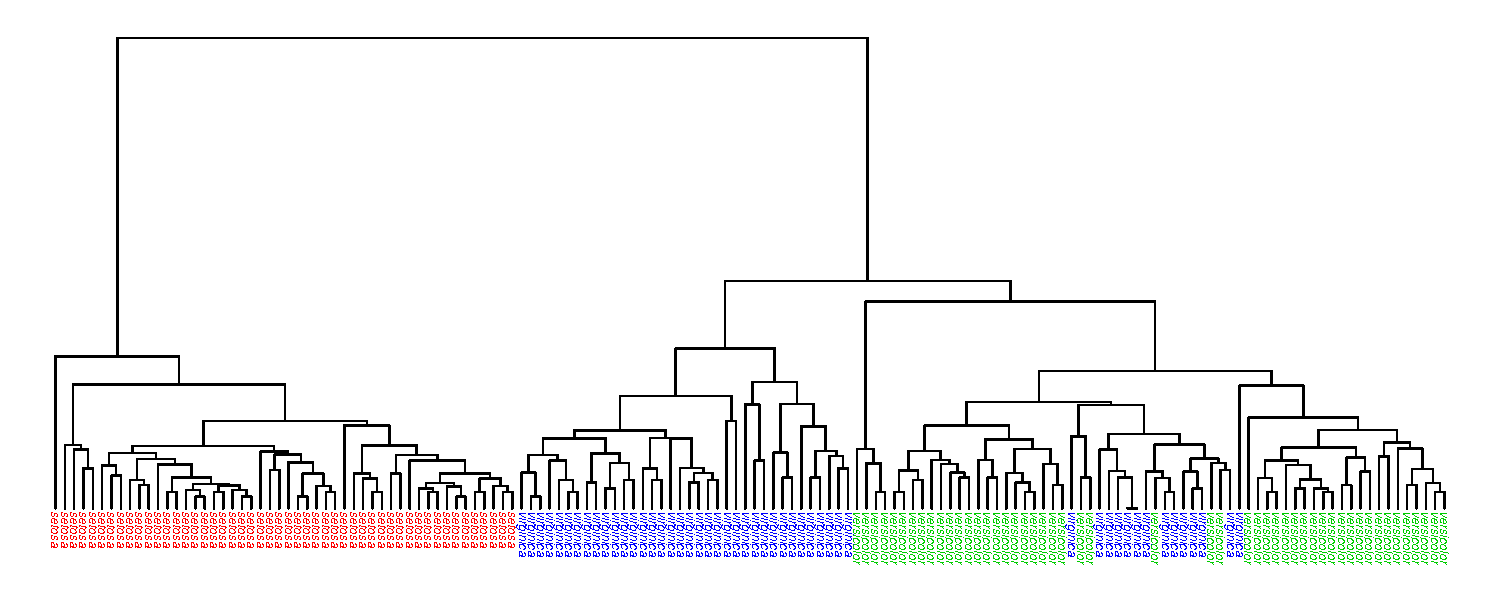
\includegraphics[width=5.5in]{pbdDEMO-include/pics/dist_iris}
% \caption{Hierarchical clustering result of \code{iris} dataset.}
% \label{fig:dist_iris}
% \end{figure}


\section{Phylogenetic Tree}

In some sense, Figure~\ref{fig:dist_iris} is an rooted tree and the
``average'' method as well as UPGMA assumes a constant rate of evolution
(molecular clock hypothesis). However, these assumption may not be
appropriate to most biological topics.



\section{Exercises}
\label{sec:pairwise_exercise}

\begin{enumerate}[label=\thechapter-\arabic*]

\item
Prove that clustering based on Euclidean distance is equivalent to that
clustering based on multivariate Normal distributions with identity variance
covariance matrices.

\item
Prove that the ``average'' method of \code{hclust()} is equivalent to the
UPGMA method.

\end{enumerate}

